\documentclass{article}
\usepackage{tempora}
\usepackage{indentfirst}
\usepackage{tabularx}
\usepackage{caption}
\usepackage{graphicx}
\usepackage{longtable}
\usepackage{tabularx}
\usepackage{amsmath}
\usepackage{amsfonts}
\usepackage{floatrow}
\floatsetup[table]{capposition=top}
\makeatletter
\graphicspath{ {./images/} }
\renewcommand*\l@section{\@dottedtocline{1}{1.5em}{2.3em}}
\makeatother
\usepackage{float}
\usepackage[english, russian]{babel}
\begin{document}
  \textbf{Постановка задачи}.

  Решается задача поиска оптимального распределения функционала программного средства по плагинам для интеграции в плагинную систему с уменьшенем связности его компонентов. При этом существуют ограничения на общее число используемых плагинов и на распределение функционала по ним. Функционал описан в требованиях к программному средству и реализован в файлах исходного кода на языке программирования.

  Определим три множества элементов предметной области:
  \begin{enumerate}
    \item $R^*$ - множество всех описанных требований
    \item $F^*$ - множество всех файлов исходного кода
    \item $P^*$ - множество всех доступных плагинов
  \end{enumerate}

  Количество элементов, которые эти множества содержат, будем обозначать так:
  \begin{itemize}
    \item $n = |R^*|$ - общее количество всех описанных требований
    \item $m = |F^*|$ - общее количество всех файлов исходного кода
    \item $k = |P^*|$ - общее количество всех доступных плагинов
  \end{itemize}

  Задача накладывает следующие ограничения на элементы множеств:
  \begin{itemize}
    \item $\forall r (r \in R^* \quad \exists f : f \in F^*(r))$ - каждое требование трассируемо по меньшей мере на один файл
    \item $\forall f (f \in F^* \quad \exists r : r \in R^*(f))$ - каждый файл реализует по меньшей мере одно требование
    \item $\forall p (p \in P^* \quad \exists f : f \in F(p))$ - каждый плагин содержит по меньшей мере один файл
    \item $\forall f (f \in F^* \quad \exists p : p = P^*(f))$ - каждый файл включен в плагин, причем единсвенный раз
  \end{itemize}

  Для формирования поставки программного средства все функциональные зависимости должны быть разрешены без появления циклических зависимостей между плагинами.

  Для описания ограничений математической модели с учетом вышесказанного введем дополнительные обозначения:

  \begin{itemize}
    \item $C^*$ - множество возможных комплектаций при заданном распределении функционала по плагинам
    \item $P'$ - множество плагинов в рамках поставки
    \item $P^D$ - множество плагинов, на которые существует зависимость у $p$
  \end{itemize}

  Для формирования поставки необходимо выполнение следующих условий:
  \begin{itemize}
    \item $\forall p (p \in P' \implies P^D_i(p) \subset P')$ - все зависимости поставляемых плагинов должны быть разрешены в рамках поставки
    \item $\forall p (p \in P' \implies p \not \in C(P^D(p)))$ - циклические зависимости между плагинами недопустимы
  \end{itemize}

  Заметим, что максимальное значение $|C^*|$ составляет $2^k - 1$ и возможно при выполнении следующего условия:
  
  $\forall p (p \in P^* \implies P^D_i(p) = \emptyset)$ - если у плагинов отсутствуют зависимости друг на друга
  
  Связь между элементами описываемой модели удобно описать при помощи графа $G = \langle V, E \rangle$

  \begin{figure}[H]
      \centering
      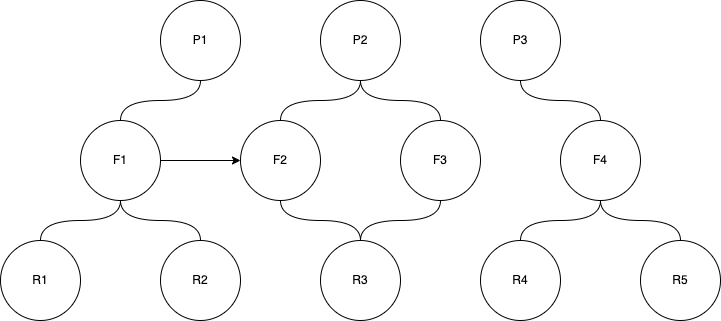
\includegraphics[width=1\textwidth]{Исходный граф.drawio}
      \caption{Граф $G$}
  \end{figure}
  
  \begin{itemize}
    \item $V = R^* \cup F^* \cup P^*$ - множество всех вершин графа
    \item $E = e_{F, R} \cup e_{P, F} \cup e_{F, F} \cup e_{P, P}$ - множество всех ребер графа
    \begin{itemize}
      \item $e_{F, R} = \bigcup^m_i \bigcup^n_j e_{f_i, r_j}$ - часть ребер отображающих трассируемость требований на файлы исходного кода. Направлений не имеют \\
      $
        e_{f_i, r_j} =
        \begin{cases}
          \{f_i, r_j\} & \text{ если } r_j \text{ трассируемо на } f_i \\
          \emptyset & \text{ если } r_j \text{ не трассируемо на } f_i
        \end{cases}
      $
      \item $e_{P, F} = \bigcup^k_i \bigcup^m_j e_{p_i, f_j}$ - часть ребер отображающих распределение файлов исходного кода по плагинам. Направлений не имеют \\
      $
        e_{p_i, f_j} =
        \begin{cases}
          \{p_i, f_j\} & \text{ если } f_j \text{ относится к } p_i \\
          \emptyset & \text{ если } f_j \text{ не относится к } p_i
        \end{cases}
      $
      \item $e_{F, F} = \bigcup^m_i \bigcup^m_j e_{f_i, f_j}$ - часть ребер отображающих зависимость файлов исходного кода друг на друга. Имеют направление \\
      $
        e_{f_i, f_j} =
        \begin{cases}
          \{f_i, f_j\} & \text{ если } f_j \text{ имеет зависимость на } f_i \\
          \emptyset & \text{ если } f_j \text{ не имеет зависимость на } f_i
        \end{cases}
      $
      \item $e_{P, P} = \bigcup^k_i \bigcup^k_j e_{p_i, p_j}$ - часть ребер отображающих зависимость плагинов друг на друга. Имеют направление \\
      $
        e_{p_i, p_j} =
        \begin{cases}
          \{p_i, p_j\} & \text{ если } p_j \text{ имеет зависимость на } p_i \\
          \emptyset & \text{ если } p_j \text{ не имеет зависимость на } p_i
        \end{cases}
      $
    \end{itemize}
  \end{itemize}

  Зависимость между плагинами образуется если:

  $ \exists (f1, f2) \in F^* :
    \begin{cases}
      e_{f_1, f_2} = \{f_1, f_2\} \\
      P^*(f1) \not = P^*(f2)
    \end{cases}
  $ 

  - если между двумя файлами есть зависимость и файлы распределены по разным плагинам

  Поставка программного средства выполняется с целью включения в нее всего полезного для заказчика функционала. Общий объем поставки дополнительно к полезному функционалу может содержать еще и бесполезный функционал. Это происходин из-за наличия вышеописанных функциональных зависимостей между компонентами программного средства. Критерием приближения к оптимальности декомпозиции функционала по плагинам является уменьшение доли бесполезного функционала для заказчика в рамках возможных поставок.

  Введем следующие обозначения:
  \begin{itemize}
    \item $R'$ - множество поставляемых требований
    \item $R_n$ - множество полезных требований в рамках поставки
    \item $R_{un}$ - множество бесполезных требований в рамках поставки
    \item $K_{un}$ - коэффициент бесполезности
  \end{itemize}

  Коэффициент бесполезности - это доля бесполезного функционала для заказчика в поставке. В рамках данной задачи этот показатель является определяющим фактором по оценке эффективности декомпозиции функционала. Для его вычисления необходимо:
  \begin{itemize}
    \item $R' = \bigcup P^*(F^*(r)) \quad \forall r (r \in R_n)$ - вычислить общий объем поставляемых требований
    \item $R_{un} = R' \setminus R_n$ - определить бесполезные требования в рамках поставки
    \item $K_{un} = \frac{|R_{un}|}{|R'|}$ - рассчитать значение коэффициента
  \end{itemize}
  
  Рассчет этого значения для определенного варианта поставки непоказателен. Для оценки того, что он изменился и в какую сторону необходимо выполнить расчеты для разных комплектаций с различным потребным функционалом. Для простоты в рамках задачи я планирую объединять требования в группы по их отношению к тому или иному конфигурируемому параметру.

  В результате планируется получить два вектора коэффициентов бесполезности: до и после. Затем проводить анализ эффективности по таким величинам как: среднее значение, математическое ожидание, среднеквадратичное отклонение и т.д.

\end{document}
